\chapter{親子の身長の研究}
% https://twitter.com/ynakahashi1003/status/1610952694767968257

% https://twitter.com/ynakahashi1003/status/1610951312560238594
%参照元の記事、モデルと推定法が区別できてないように感じるし、「線形回帰モデルは実際にこの方法で回帰係数を推定しています」という記述もどんなソフトウェアのどんな関数なのかも書いてなくて正直微妙だなぁ、と。例えばRのlmがあれを計算してるかって言ったらしてないでしょ
\begin{comment}
https://twitter.com/Yh_Taguchi/status/1589082783577944064

https://mathlog.info/articles/2936
https://jp.quora.com/%E7%9B%B8%E9%96%A2%E4%BF%82%E6%95%B0%E3%81%8C0-8%E3%81%A8%E3%82%8F%E3%81%8B%E3%81%A3%E3%81%A6%E3%81%84%E3%82%8B%E9%96%A2%E4%BF%82%E3%82%92%E4%BD%BF%E3%81%A3%E3%81%A6%E7%9B%B8%E9%96%A2%E4%BF%82%E6%95%B01%E3%81%A8/answers/325575293
https://www.jstage.jst.go.jp/article/jve/25/1/25_51/_pdf/-char/ja
https://journals.biologists.com/jeb/article/125/1/29/5000/Fracture-Toughness-Design-In-Horse-Hoof-Keratin?searchresult=1#11919084
https://journals.biologists.com/jeb/article/199/6/1295/7289/The-Effects-of-Salinity-Change-on-the-Exercise?searchresult=1#12304883
https://journals.biologists.com/jeb/article/191/1/19/6760/Variations-in-Force-Time-Histories-of-cat?searchresult=1#13965593
https://www.jstage.jst.go.jp/article/jve/24/1/24_29/_pdf/-char/ja 
\end{comment}

二つの要素に対する3つのモデルを取り上げる。まず、これらの性質について整理する。

\section{独立ではない変数を持つモデル}
\begin{enumerate}
 \item $x,y$を確率変数とする。
 \item 平均を$\mu_x,\mu_y$分散を$\sigma^2_x,\sigma^2_y$とする。
\end{enumerate}
このモデルでは、次の$X$と$Y$の共分散という量が定義できる。
\begin{equation*}
 \sigma_{xy} = E[(x-\mu_x)(y-\mu_y)]
\end{equation*}
また、相関係数を次のように定義する。
\begin{equation*}
 \rho = \frac{\sigma_{xy}}{\sigma_x\sigma_y}
\end{equation*}

$(x-\mu_x)(y-\mu_y)$という量を考えてみる。これは$(\mu_x,\mu_y)$を中心にし、
\begin{enumerate}
 \item $(x,y)$が右上にあれば、$x-\mu_x$と$y-\mu_y$はともに正であり、その積も正
 \item $(x,y)$が左下にあれば、$x-\mu_x$と$y-\mu_y$はともに負であり、その積は正
 \item $(x,y)$が左上にあれば、$x-\mu_x$は負そして、$y-\mu_y$は正であり、その積は負
 \item $(x,y)$が右下にあれば、$x-\mu_x$は正そして、$y-\mu_y$は負であり、その積は負
\end{enumerate}
である。以上から、$(x-\mu_x)(y-\mu_y)$は2次元平面上でのある中心からデータのばらつき方を示す量であること、
そして、その平均は、平均的なデータのばらつきかたを示す。言い替えれば、平均的にデータが$(\mu_x,\mu_y)$を中心に右上から左下に多く存在すれば、共分散は正の値をとることが期待される。
共分散を$\sigma_x,\sigma_y$により規格化した量が相関係数である。

相関係数は、二つの変数が確率変数であることを仮定したモデルにより定義できる量である。


\subsection{$r^2\leq 1$の証明}
コーシーシュワルツの不等式
$a_1,a_2,\cdots,a_n,b_1,b2,\cdots,b_n$を実数とする。
\begin{equation*}
 (\sum_{i=1}^n a_i b_i)^2 \leq (\sum_{i=1}^n a_i^2)(\sum_{i=1}^n b_i^2)
\end{equation*}
である。等号成立は、$a_i=0$または$b_i=0$または$b_1/a_1=b_2/a_2=\cdots=b_n/a_n$が成り立つときである。

このことを利用する。$a_i=x_i-\bar{x},b_i=y_i-\bar{y}$とおく。
\begin{equation*}
 \left(\sum_{i=1}^n (x_i-\bar{x})(y_i-\bar{y})\right)^2 \leq  \sum_{i=1}^n(x_i-\bar{x})^2\sum_{i=1}^n(y_i-\bar{y})^2
\end{equation*}
このことから、$r^2\leq 1$であり、$-1\leq r \leq 1$がわかる。


\section{$2$変量正規分布}
独立ではない二つの変数に対するモデルを構築する。
\begin{enumerate}
 \item $(x_i,y_i)\sim F (i=1,2,\cdots,n)$
 \item $F$は$2$変量正規分布
 \item 母数は、平均値、分散および共分散
\end{enumerate}
このモデルを$2$変量モデル$M_{2}(\mu,\sum)$と呼ぶ。
このモデルの最尤推定量は次の通り。
\begin{eqnarray*}
 \mu &=& \left(\frac{1}{n}\sum_{i=1}^n x_i,\frac{1}{n}\sum_{i=1}^n y_i \right) \\
 \sum &=& \begin{pmatrix}
\frac{1}{n}\sum (x_i-\bar{x})^2 &  \frac{1}{n}\sum (x_i-\bar{x})(y_i-\bar{y})\\
\frac{1}{n}\sum (x_i-\bar{x})(y_i-\bar{y}) & \frac{1}{n}\sum (y_i-\bar{y})^2 \\
\end{pmatrix}
\end{eqnarray*}

$x_1$または$x_2$を固定したときに得られる、$x_2$または$x_1$の期待値と分散は次の通り。
\begin{eqnarray*}
 E[x_2|x_1] &=& \mu_2+\frac{\sigma_{xy}}{\sigma_x^2}(x_1-\mu_1)\\
 Var[x_2|x_1]  &=& \sigma_2^2(1-\rho^2) \\
 E[x_1|x_2] &=& \mu_1+\frac{\sigma_{yx}}{\sigma_y^2}(x_2-\mu_2)\\
 Var[x_1|x_2]  &=& \sigma_1^2(1-\rho^2)
\end{eqnarray*}
$E[x_2|x_2]$を$x_2$の$x_1$に対する回帰という。
この式は、平均二乗誤差を最小にするという良い性質をもっている。



正規2モデル$M(\mu_x,\mu_y,\sigma_x^2,\sigma_y^2)$において、相関係数が次の分布に従う。
\begin{equation*}
 r \sim 
\end{equation*}
このことを利用して、データと正規2モデルとの乖離具合を調べることができる。
これは、相関係数に対する検定と呼ばれる作業に対応する。


\section{誤差モデルI}
ここで、誤差項が確率変数であることを仮定してモデルModel Iを構築する。
\begin{enumerate}
 \item $x_i$は、与えられた定数
 \item $a,b$を実数の定数
 \item $u_i = y_i-a x_i -b$
 \item $u_i \sim N(0,\sigma^2)$
 %\item $E[u_i]=0$。平均は$0$。
 %\item $E[u_j u_i]=0$。無相関。
 %\item $Var[u_i]=0$。分散が均一。
\end{enumerate}
この仮定により構築されるモデルを$M_{I}(a,b; x)$または$M_I(a,b)$と表記する\footnote{正規性の仮定の代わりに、無相関、等しい分散、平均が$0$の仮定を与えるのが簡単な定義である。ここでは、正規性を仮定しておいた}。
また、最尤推定量を挿入した最尤モデルを$M_I(\hat{a},\hat{b})$と表記する。
この最尤推定量は次の通りである。
\begin{eqnarray*}
 \hat{a} &=& \frac{Q_{xy}}{Q_{xx}}\\
 \hat{b} &=& \bar{y}-\hat{a}\bar{x}
\end{eqnarray*}
予測値と観測値の差分を残差$e_i$、またその二乗和を残差平方和とよぶ。それぞれ、以下の通り。
\begin{eqnarray*}
 e_i &=& y_i - (ax_i+b)\ \ (i=1,2,\cdots,n)\\
 RSS &=& \sum_{i=1}^n e_i^2 \\
\end{eqnarray*}
そして分散の推定値を以下のように定義する。
\begin{eqnarray*}
 \hat{\sigma}^2 = \frac{RSS}{n-2}
\end{eqnarray*}
モデル$M_I(a,b)$において、次のことも解っている。
\begin{equation*}
 \frac{(\hat{a}-a)}{ \left( \frac{\hat{\sigma}^2}{Q_{xx}} \right)^\frac{1}{2}} \sim t_{n-2}
\end{equation*}
また、このことから、$a$の信頼区間は、次の通り。
\begin{equation*}
 |a| \leq \hat{a}\pm(\hat{\sigma}^2/Q_{xx})^{1/2}t_{n-2,\frac{\alpha}{2}}
\end{equation*}
$y$の予測区間は、以下の通りである。
\begin{equation*}
 y_0\pm\left[\hat{\sigma}^2\left( 1+\frac{1}{n} +\frac{(x_0-\bar{x})^2}{Q_{xx}} \right)\right]^{1/2}t_{n-2,\alpha/2}
\end{equation*}

\subsection{決定係数$R^2$と相関係数$\rho^2$の関係}
この誤差モデルにおいて、決定係数$R^2$と相関係数$\rho^2$の関係を調べる。
まず、最尤推定した$\hat{a},\hat{b}$を用いて、残差平方和の計算をおこなう。
\begin{eqnarray*}
 \sum_{i=1}^n e_i^2 &=&  \sum_{i=1}^n ((y_i-\bar{y})-\frac{\sigma_{xy}}{\sigma^2_x}(x_i-\bar{x})^2)\\
 &=& n\sigma^2_y -n \frac{\sigma^2_{xy}}{\sigma_x^2} \\
 &=& n\sigma_y^2(1-\frac{\sigma^2_{xy}}{\sigma^2_x\sigma_y^2}) \\
 &=& n\sigma_y^2(1-\rho^2)
\end{eqnarray*}
以上より、平均二乗誤差は、以下とも等しい。
%ここで、回帰平均二乗誤差RMSE(regression mean square)を定義しておく。
\begin{equation*}
 %RMSE^2 = 
 RSS = (\sigma_y\sqrt{1-\rho^2})^2
\end{equation*}
このことを用いて、決定係数$R^2$について計算を行う。
\begin{eqnarray*}
 R^2 &=& 1-\frac{\sum_{i=1}^n e_i^2}{\sum_{i=1}^n (y_i-\bar{y})^2} \\
 &=& 1-\frac{n\sigma_y^2(1-\rho^2)}{n\sigma^2_y} \\
 &=& \left( \frac{\sigma_{xy}}{\sigma_x\sigma_y}\right)^2 = \rho^2
\end{eqnarray*}

誤差モデルにおいては、決定係数と相関係数の二乗が一致することがわかる。
このことから誤差モデルにおいては、決定係数は$0\leq R^2\leq 1$であることがわかる。
%このように計算をおこなわなくても、誤差モデルにおいて$0\leq R^2\leq 1$が成立することは、平均値よりも予測がわるくなることはなさそうであるので、$0\leq R^2$は明らか。

\paragraph{決定係数の意味}
決定係数は、平均値による予測と比べて、提案した誤差モデルでの予測がどれくらい良くなったのかを示す指標である。
第二項は、分母に、平均と観測値の差の二乗、分子に予測値と観測値の差の二乗をしたものである。

\subsection{独立な2変数モデルの回帰平均二乗誤差}
ここで、正規モデル$M(\mu,\sigma)$を正規モデル$M'(\mu,\sigma)$により予測することを考える。
モデル$M,M'$での確率変数をそれぞれ$x,y$とする。$x$を$y$により予測したとき、その誤差を計算する。
\begin{equation*}
 RMSE^2 = \frac{1}{n}\sum_{i=1}^n (x_i-y_i)^2
\end{equation*}

\begin{eqnarray*}
 RMSE^2=\frac{1}{n}\sum_{i=1}^n (x_i-y_i)^2 &=& \frac{1}{n}\sum_{i=1}^n \left( (x-\mu)-(y-\mu)\right) ^2\\
 &=& \frac{1}{n}\sum_{i=1}^n (x-\mu)^2+\frac{1}{n}\sum_{i=1}^n(y_i-\mu)^2-\frac{2}{n}\sum_{i=1}^n(x_i-\mu)(y_i-\mu) \\
 &=& Var[x]+Var[y]-2cov[x,y] \\
 &=& 2Var[x]
\end{eqnarray*}
以上より、
\begin{equation*}
 RMSE_{random} = \sqrt{2}\sigma
\end{equation*}
がわかる。
これは、確率変数を別の確率変数により予測しようとすると、二乗誤差は分散の$\sqrt{2}$倍である\footnote{平均により予測すると、二乗誤差は$\sigma$なので、この予測モデルはそれよりも悪い。}。

\subsubsection{決定係数が負になる}
以上の議論を踏まえ、決定係数が負になることをみておこう。
\begin{eqnarray*}
 R^2 &=& 1-\frac{\sum_{i=1}^n (x_i-y_i)^2}{\sum_{i=1}^n (x_i-\bar{x})^2}\\
 &=& 1-\frac{2n\sigma}{n\sigma}\\
 &=& -1
\end{eqnarray*}
平均値より予測精度が悪いことを決定係数が示している。


\subsection{相関係数が$0.8$のとき}
相関係数が$0.8$のとき、$RMSE$は、$RMSE^2 = \sigma_y\sqrt{1-\rho^2}$より、
\begin{equation*}
 RMSE = 0.6\sigma
\end{equation*}
である。
これは、回帰により二乗誤差が$\sigma$からその$0.6$倍改善されたことを示している。
また、確率変数による予測は$\sqrt{2}\sigma$なので、このモデルと比較すると、
\begin{equation*}
 0.6\sigma = 0.428(\sqrt{2})\sigma
\end{equation*}
より、$0.42倍$改善されている\footnote{https://mathlog.info/articles/2936}
ランダムモデルの$RMSE$の$58\%$割引ともいえる。


\section{誤差モデルII}
$x$に対する予測値との差が正規分布にしたがうことを仮定したモデルも構築する。
\begin{enumerate}
 \item $y_i$は、与えられた定数
 \item $a,b$を実数の定数
 \item $v_i = \frac{1}{a}(y_i-a x_i -b)$
 \item $v_i \sim N(0,\sigma^2)$
 %\item $E[u_i]=0$。平均は$0$。
 %\item $E[u_j u_i]=0$。無相関。
 %\item $Var[u_i]=0$。分散が均一。
\end{enumerate}



\section{親子の身長の関係}


PearsonとLeeらによる親と子供の身長に関するデータを利用した\footnote{\url{https://vincentarelbundock.github.io/Rdatasets/datasets.html}}。
\begin{table}[http]
 \centering
 %父と息子の統計量を要約したもの
 \begin{tabular}{lrr}
  {} &  子供 &  親 \\
  個数 & 179 &  179 \\
  平均  &  68.33 &   67.08 \\
  標準偏差   &   4.53 &    4.03 \\
  最小値   &  59.50 &   58.50 \\
  25\%   &  64.50 &   64.00 \\
  50\%   &  68.50 &   67.50 \\
  75\%   &  71.50 &   70.50 \\
  最大値   &  78.50 &   74.50 \\
 \end{tabular}
\end{table}


\begin{table}[http]
 \centering
\begin{tabular}{lrr}
{} &    $\hat{a}$ &      $\hat{b}$ \\
$E_1$ & 0.59 &  29.02 \\
 $E_2$ & 2.16 & -76.69 \\
$E_3$ & 1.25 & -15.76 \\
$E_4$ & 1.13 &  -7.18 \\
\end{tabular}
\end{table}




\if 0
\section{Model I}




\begin{comment}
これはちがう
 with pm.Model() as model1:  # model specifications in PyMC are wrapped in a with-statement
    # Define priors
    xdata = pm.ConstantData("x", x, dims="obs_id")

    sigma = pm.HalfCauchy("sigma", beta=20)
    #sigma = pm.Uniform("sigma",lower=10**-3,upper=10**3)

    intercept = pm.Normal("intercept", 0, sigma=100)
    #intercept = pm.Beta("intercept",alpha=5,beta=1)
    slope = pm.Normal("slope", 0, sigma=100)
    #intercept = pm.Uniform("intercept",lower=10**-3,upper=10**3)

    #slope = pm.Uniform("slope",lower=10**-3,upper=10**3)

    # Define likelihood
    #likelihood = pm.Normal("y", mu=intercept + slope * xdata, sigma=np.sqrt(slope)*sigma, observed=y)
    #likelihood = pm.Normal("y", mu=intercept + slope * xdata, sigma=sigma/np.sqrt(1+slope**2), observed=y)
    likelihood = pm.Normal("y", mu=(intercept + slope * xdata), sigma=sigma, observed=y)
    # Inference!
    # draw 3000 posterior samples using NUTS sampling
    idata = pm.sample(3000,cores=3)
\end{comment}
\fi

\if 0
\section{Model I'}
実数のペア$(x_1,y_1),(x_2,y_2),\cdots,(x_n,y_n)$が次の線形な関係を持つとする。
\begin{comment}
\begin{equation*}
 u_i =x_i -\frac{y_i-a}{b} \ \ (i=1,2,\cdots,n)
\end{equation*} 
\end{comment}
ここで、誤差項が確率変数であることを仮定してモデルModel I'を構築する。
\begin{enumerate}
 \item $x_i$は、与えられた定数
 \item $a,b$を実数の定数
 \item $u_i = x_i -\frac{y_i-b}{a}$
 \item $u_i \sim N(0,\sigma^2)$
 %\item $E[u_i]=0$。平均は$0$。
 %\item $E[u_j u_i]=0$。無相関。
 %\item $Var[u_i]=0$。分散が均一。
\end{enumerate}
この仮定により構築されるモデルを$M_{I'}(a,b; x)$または$M_{I'}(a,b)$と表記する

\subsection{尤度}
このモデルの対数尤度のうち、
\fi
\begin{comment}
 with pm.Model() as model1:  # model specifications in PyMC are wrapped in a with-statement
    # Define priors
    ydata = pm.ConstantData("y", y, dims="obs_id")

    sigma = pm.HalfCauchy("sigma", beta=10)
    #sigma = pm.Uniform("sigma",lower=10**-3,upper=10**3)

    intercept = pm.Normal("intercept", 0, sigma=100)
    #intercept = pm.Beta("intercept",alpha=5,beta=1)
    slope = pm.Normal("slope", 0, sigma=100)
    #intercept = pm.Uniform("intercept",lower=10**-3,upper=10**3)

    #slope = pm.Uniform("slope",lower=10**-3,upper=10**3)

    # Define likelihood
    likelihood = pm.Normal("x", mu=(ydata-intercept)/slope, sigma=sigma, observed=x)

    # Inference!
    idata = pm.sample(3000,cores=3)
\end{comment}

\if 0
\section{Model II'}

\begin{enumerate}
 \item $x_i-u_i \sim N(0,\sigma^2)$
 \item $y_i-v_i \sim N(0,\sigma^2)$
 \item $a,b$を実数の定数
 \item $v_i -a u_i -b = 0$
\end{enumerate}
この仮定により構築されるモデルを$M_{II'}(a,b; x)$または$M_{II'}(a,b)$と表記する

\subsection{最尤モデル}
このモデルの尤度を計算する。
\begin{eqnarray*}
 L &=& \prod_{i=1}^{n}\frac{1}{\sqrt{2\pi\sigma^2}}\exp\left(-\frac{(x_i-u_i)^2}{2\sigma^2} \right)\prod_{i=1}^{n}\frac{1}{\sqrt{2\pi\sigma^2}}\exp\left(-\frac{(y_i-v_i)^2}{2\sigma^2} \right)\\
 &=& \prod_{i=1}^{n}\frac{1}{\sqrt{2\pi\sigma^2}}\exp\left(-\frac{(x_i-u_i)^2+(y_i-v_i)^2}{2\sigma^2} \right)
\end{eqnarray*}
対数尤度で、

\subsection{モデルの拡張}
このモデルは、次の様に、誤差の分散について拡張できる。
\begin{enumerate}
 \item $x_i-u_i \sim N(0,\sigma_x^2)$
 \item $y_i-v_i \sim N(0,\sigma_y^2)$
 \item $a,b$を実数の定数
 \item $v_i -a u_i -b = 0$
\end{enumerate}
このモデルの最尤推定量は、上記と同様のはずなので、詳しくは計算を行わない。
\begin{eqnarray*}
 \hat{a} &=& \frac{Q_{yy}-\lambda Q_{xx}+\sqrt{(Q_{yy}-\lambda Q_{xx})^2+4\lambda Q_{xy}}}{2Q_{xy}} \\
 \hat{b} &=& \bar{y}-\hat{a}\bar{x}
\end{eqnarray*}
ここで、$\lambda = \frac{\sigma_x^2}{\sigma_y^2}$である。


\fi




\begin{comment}
 \begin{table}
 \begin{tabular}{llll}
  名前 & 最小化要素 & 最小化関数 & \\
  \hline \hline\\
  Model I regression & && \\

  Regression &$y$軸方向の変動を最小化 & $s_{y,x}(\Delta y^2)$ & \\
  Model II regression & && \\

  標準主軸回帰 &  $x,y$軸方向から直線への変動を最小化 & $\Delta x\Delta y$ &  \\
  standard major axis(SMA回帰) &&& \\
  major axis regression, &&& \\
  幾何平均回帰, Reduced major axis(RMA) &&& \\
  主成分分析(Principal component analysis) &観測点$(x,y)$から直線への最短距離を最小化 & $s\Delta h^2$ & \\

  %Deming回帰 &  & $s_d$ & \\
 \end{tabular}
\end{table}

幾何平均回帰は,標準化主軸回帰(Standardised major axis(SMA回帰))標準主軸 (Standard major axis)回帰,縮小長軸(Reduced major axis, RMA)回帰
Principal component analysis 主成分回帰は,主軸回帰,最大軸回帰 MA(Major axis), Orthogonal regression


\begin{table}
 \begin{tabular}{llll}
  名前 & 最小化要素 & 最小化関数 & \\
  \hline \hline
  Model I regression & && \\

  Regression &$y$軸方向の変動を最小化 & $s_{y,x}(\Delta y^2)$ & \\
  Model II regression & && \\

  SMA回帰 &  $x,y$軸方向から直線への変動を最小化 & $\Delta x\Delta y$ &  \\
  PCA &観測点$(x,y)$から直線への最短距離を最小化 & $s\Delta h^2$ & \\

  %Deming回帰 &  & $s_d$ & \\
 \end{tabular}
\end{table}

\end{comment}




\section{観測点を直線により予測する}
実数のペア$(x_1,y_1),(x_2,y_2),\cdots,(x_n,y_n)$が次の線形な関係を持つとする。
\begin{equation*}
 y_i = ax_i+b+u_i, \ \ (i=1,2,\cdots,n)
\end{equation*}

点A$(x,y)$と直線の関係を図\ref{fig:RegressionModel}に示しす。
点$A$と同じ$x$座標の直線上の点$D$は、$(x,ax+b)$である。
点$A$と同じ$y$座標の直線上の点$B$は、$(\frac{y-b}{a},y)$である。
$DA$間の距離を$|\Delta y$、$BA$間の距離を$|\Delta x|$で表す。
$BA$間の距離は、$|\Delta x| = \frac{|\Delta y|}{a}$である。
これは、
\begin{eqnarray*}
 \Delta x &=& x-\frac{y-b}{a} \\
 &=& \frac{ax+b-y}{a} \\
 &=& \frac{\Delta y}{a}
\end{eqnarray*}
より明らかである。
また、点$A$から直線に向けて垂直に下した点を$C$とする。
$AC$間の距離は、$\frac{|y-ax-b|}{\sqrt{a^2+1}}$である。
また、三角形$ABD$の面積の倍は$\Delta x\Delta y =\frac{\Delta x^2}{a}$である。


\begin{figure}
 \begin{center}
  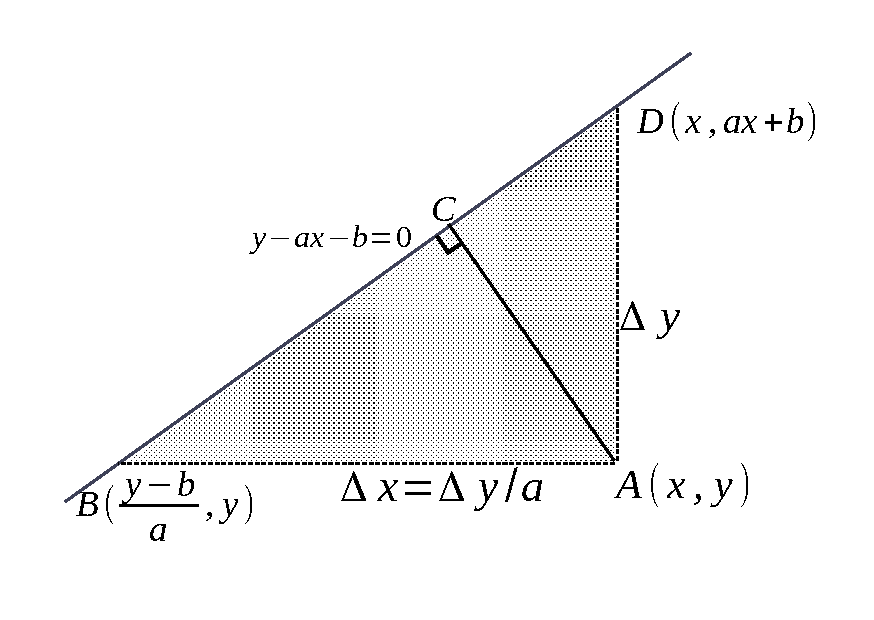
\includegraphics[width=8cm]{./image/16_/RegressionModel.pdf}
  \caption{点$A$と直線$Y=aX+b$の関係}
  \label{fig:RegressionModel}
 \end{center}
\end{figure}

以上から点と直線の距離について4つの方法で定義ができることがわかる。
また、各点についてそれぞれの式を和にすると、以下の通りである。
\begin{enumerate}
 \item 点と直線の最短距離$AC$:$E_3 = \sum (\frac{\Delta y_i}{\sqrt{1+a^2}})^2$
 \item $y$軸に関する距離$AD$:$E_1=\sum \Delta y_i^2$
 \item $x$軸に関する距離$AB$:$E_2=\sum  (\frac{\Delta y_i}{a})^2=\sum (\Delta x)^2$
 \item 面積を元にした距離$AB\times AD$:$2\times E_4 = \sum (\frac{\Delta y_i}{\sqrt{a}})^2$
\end{enumerate}

ある点と直線への距離が離れていれば、その点への予測ができていないことを示し、近ければ、それなりによい予測をしているだろう。
このことから、$E_j$が小ければ、それぞれの距離の意味で、各々の点と直線が近いはずである。
そこで、まず$E_j$が最も小さくなるように直線のパラメータ$(a_j,b_j)(j=1,2,3,4)$を定める。
さらに、それぞれの直線の性質についてしらべる。


\paragraph{点と直線の最短距離}
点と直線の距離について証明を行う。大抵の高校数学の教科書には記述されているはずである。
点$A(x,y)$から直線$Y-aX-b=0$への直線距離$d$の関係を求める。
点$B$は、点$A$を$x$方向に移動させたとき、直線と交わる点である。つまり点$B$は、$(\frac{y-b}{a},y)$である。
また点$D$は、点$A$を$y$方向に移動させたとき、直線と交わる点である。つまり点$D$は、$(x,ax+b)$である。
点$C$は、点$A$を直線$Y-aX-b=0$へ垂直に下ろした点である。この$AC$間の距離を$d$とする。
直線$DA$と直線$AC$のなす角度を$\theta$とする。
このとき、次の関係が求められる。
\begin{eqnarray*}
 \sin \theta &=& \frac{AC}{BA}\\
 &=& \frac{d}{x-\frac{y-b}{a}}\\
\cos\theta &=& \frac{AC}{DA}\\
&=& \frac{d}{ax+b-y}
\end{eqnarray*}
また、$\cos^2\theta+\sin^2\theta$を計算する。
\begin{eqnarray*}
 \cos^2\theta+\sin^2\theta &=& \frac{d^2}{(y - \frac{y-b}{a})^2}+\frac{d^2}{(ax+b-y)^2}\\
 &=& \frac{d^2(a^2+1)}{(ax+b-y)^2} \\
 &=& 1
\end{eqnarray*}
この式を$d$について解く。
\begin{equation*}
 d^2 = \frac{(y-ax-b)^2}{a^2+1}
\end{equation*}


\begin{figure}
 \begin{center}
  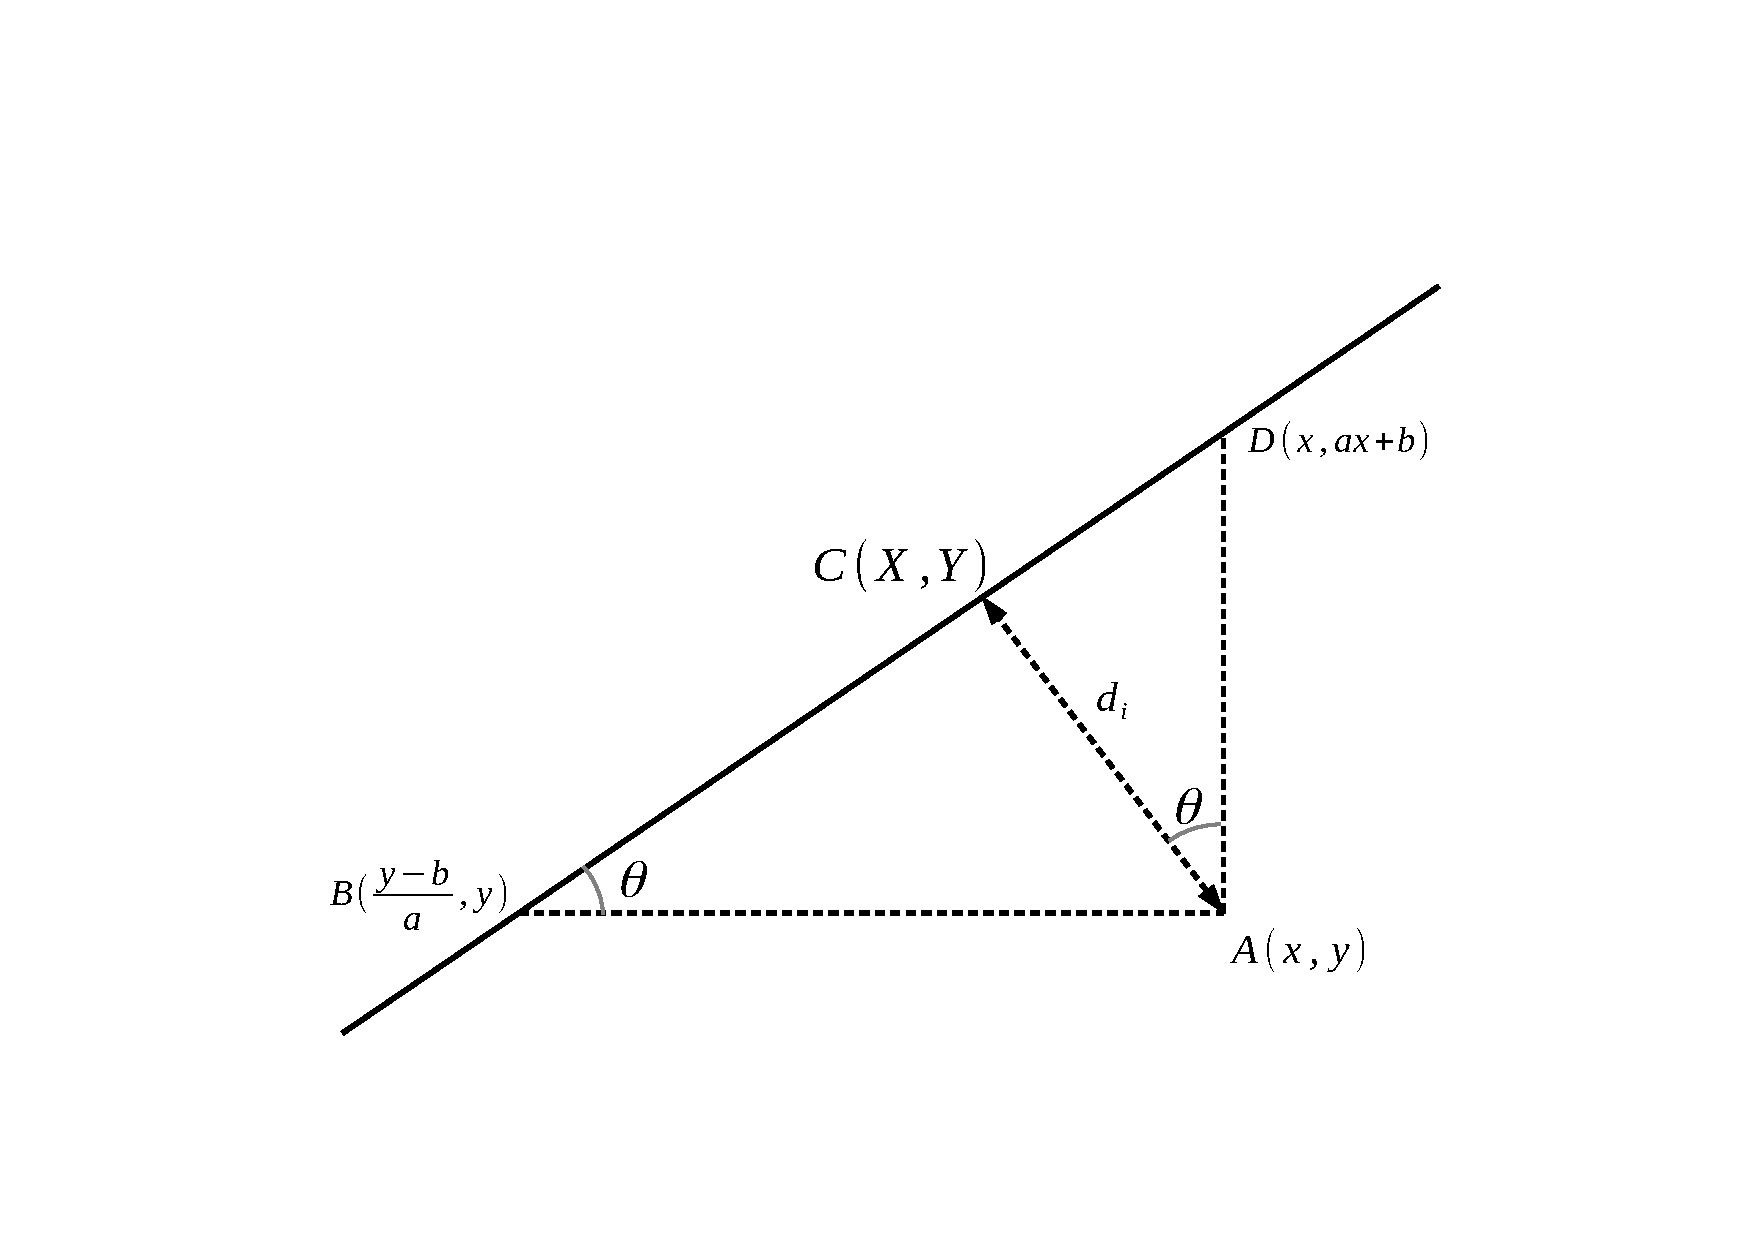
\includegraphics[width=8cm]{./image/16_/point_line_distance.pdf}
  \caption{点$A$から直線$Y=aX+b$への直線距離$d$の関係}
  \label{fig:point_line_distance}
 \end{center}
\end{figure}

\paragraph{$\sum \Delta y_i^2$に関する計算}
\begin{equation}\label{sum_square_error}
 E_1 = \sum_{i=1}^n u_i^2 = \sum_{i=1}^n (y_i-a x_i-b)^2
\end{equation}
式\ref{sum_square_error}にいくらか式変形を行う。
\begin{eqnarray*}
 \sum_{i=1}^n (y_i-a x_i-b)^2 &=& \sum_{i=1}^n \{(y_i-\bar{y}) - a(x_i-\bar{x}) +(\bar{y}-b-a\bar{x})  \}^2\\
 & =& \sum_{i=1}^n \{ (y_i-\bar{y})-a(x_i-\bar{x})  \}^2+n(\bar{y}-b-a\bar{x})^2 \\
 &=& Q_{xx}a^2-2Q_{xy}a+Q_{yy}+n(\bar{y}-b-a\bar{x})^2
\end{eqnarray*}
ここで、以下の式を定義しておく。
\begin{eqnarray*}
 \bar{x} &=& \frac{1}{n}\sum_{i=1}^n x_i \\
 \bar{y}&=& \frac{1}{n}\sum_{i=1}^n y_i \\
 Q_{xx} &=& \sum_{i=1}^n (x_i-\bar{x})^2 \\
 Q_{yy} &=& \sum_{i=1}^n (y_i-\bar{y})^2 \\
 Q_{xy} &=& \sum_{i=1}^n (x_i-\bar{x})(y_i-\bar{y}) \\
\end{eqnarray*}

\paragraph{$E_1$}
まず、式\ref{sum_square_error}を、$b$について偏微分を行う。
\begin{equation*}
 \frac{\partial E_1}{\partial b} = -2(\bar{y}-b-a\bar{x})
\end{equation*}
この式が$0$となる$b$について解くと、次が求まる。
\begin{equation*}
 \hat{b} = \bar{y}-\hat{a}\bar{x}
\end{equation*}

また、$E_1$を$a$について偏微分を行う。
\begin{eqnarray*}
 \frac{\partial E_1}{\partial a} = 2aQ_{xx}-2Q_{xy}
\end{eqnarray*}
以上から、$a$が求められる。
\begin{equation*}
 \hat{a} = \frac{Q_{xy}}{Q_{xx}}
\end{equation*}


\paragraph{$E_2$}
$a,b$に関係する部分は、以下の式である。
\begin{equation*}
 E_2 = \frac{1}{a^2}(Q_{xx}a^2-2Q_{xy}a+Q_{yy}+n(\bar{y}-b-a\bar{x})^2)
\end{equation*}
$E_2$の$b$に関する偏微分が$0$になる点は、以下の式である。
\begin{equation*}
 \hat{b} = \bar{y}-\hat{a}\bar{x}
\end{equation*}
また、$E_2$の$a$に関する偏微分を計算する。
\begin{eqnarray*}
 \frac{\partial E_2}{\partial a} &=& -\frac{2}{a^3}(a^2Q_{xx}-2Q_{xy}a+Q_{yy}) \\
& & +\frac{1}{a^2}(2aQ_{xx}-2Q_{xy})
\end{eqnarray*}
この式を$a$についてとくと、最尤推定量がもとめられる。
\begin{equation*}
 \hat{a}= \frac{Q_{yy}}{Q_{xy}}
\end{equation*}

\paragraph{$E_3$}

変数$a,b$に関連のある項を計算する。
\begin{eqnarray*}
 h(a,b) = \sum_{i=1}^n (x_i-u_i)^2+(y_i-v_i)^2
\end{eqnarray*}
対数尤度を最大化するかつ$v_i -a u_i -b = 0$を満すものを求める。

これは難しいので、幾何学的な考察を行う。
$h(a,b)$は、$(x_i,y_i)$から$(u_i,v_i)$上への距離の和を示している。これを最小化するのは、$(x_i,y_i)$から直線$v_i-a u_i-b=0$への直線距離を最小化しているのに等しい。
このことから、直線から点への距離の公式から、その和は、次の式で表すことができる。
\begin{equation*}
 E_3 = \sum_{i=1}^n \frac{ (y_i-b-ax_i)^2}{1+a^2}
\end{equation*}
$E_1$との違いは、分母に$(1+a^2)$の項が加わったことである。これが、推定量に違いを生じさせる。
式$E_3$を展開していく。
\begin{comment}
\begin{eqnarray*}
 (1+a^2)E_3 &=& \sum_{i=1}^n \{ (y_i-\bar{y})-a(x_i-\bar{x})+(\bar{y}-a\bar{x}-b) \}^2 \\
 &=& \sum_{i=1}^n \{  (y_i-\bar{y})-a(x_i-\bar{x}) \}^2+n(\bar{y}-a\bar{x}-b)^2 \\
 &=& Q_{yy}+a^2 Q_{xx}-2aQ_{xy}+n(\bar{y}-a\bar{x}-b)^2 \\
\end{eqnarray*} 
\end{comment}


\begin{equation*}
 (1+a^2)E_3 = Q_{yy}+a^2 Q_{xx}-2aQ_{xy}+n(\bar{y}-a\bar{x}-b)^2 \\
\end{equation*}
この式を最小化する。まず$b$により偏微分を行う。
\begin{eqnarray*}
 \frac{\partial E_3}{\partial b} = -2n(\bar{y}-a\bar{x}-b)
\end{eqnarray*}
これが$0$になるので、最尤推定した$\hat{b}$は次の式となる。
\begin{equation*}
 \hat{b} = \bar{y}-\hat{a}\bar{x}
\end{equation*}
次に、$a$について偏微分をおこなう\footnote{ $(f/g)'= \frac{f'g-fg'}{g^2}$ }。
\begin{eqnarray*}
\frac{\partial E_3}{\partial a} = \frac{(2aQ_{xx}-2Q_{xy})(1+a^2)-2a(Q_{yy}+a^2Q_{xx}-2aQ_{xy})}{(1+a^2)^2}
\end{eqnarray*}
分子を整理すると、次の式となる。
\begin{equation*}
 Q_{xy}a^2-a(Q_{yy}-Q_{xx})-Q_{xy}
\end{equation*}
$\frac{\partial E_3}{\partial a} =0$より、$a$について解く。
上式は、$a$に関する二次方程式なので、$a$を解く。
\begin{equation*}
 \hat{a} = \frac{Q_{yy}-Q_{xx}+\sqrt{(Q_{yy}-Q_{xx})^2+4Q_{xy}}}{2Q_{xy}}
\end{equation*}




\paragraph{$E_4$}
\begin{eqnarray*}
 E_4=\sum_{i=1}^n u_i^2 &=& \sum_{i=1}^n \frac{1}{a}(y_i-a x_i-b)^2 \\
 &=& \frac{1}{a}(Q_{xx}a^2-2Q_{xy}a+Q_{yy}+n(\bar{y}-b-a\bar{x})^2)
\end{eqnarray*}
ここで、$E_4$の$b$に関する偏微分が$0$となる$b$を求める。
\begin{equation*}
 \hat{b} = \bar{y}-\hat{a}\bar{x}
\end{equation*}
同様に、$E_4$の$a$に関する偏微分が$0$となる$a$を求める。
\begin{eqnarray*}
 \frac{\partial E_4}{\partial b} &=& \frac{1}{a}(2aQ_{xx}-2Q_{xy})\\
&& -\frac{1}{a^2}(Q_{xx}a^2-2Q_{xy}a+Q_{yy}) = 0 \\
\rightarrow && a^2 Q_{xx}-Q_{yy} = 0
\end{eqnarray*}
以上から、最尤推定量が求められる。
\begin{equation*}
 \hat{a}= \sqrt{\frac{Q_{yy}}{Q_{xx}}}
\end{equation*}
この式は、$\frac{Q_{xy}}{Q_{xx}}$と$\frac{Q_{yy}}{Q_{xy}}$の幾何平均と一致する。
ここで、幾何平均は、$0$より大きな数$a_1,a_2,\cdots,a_n$について、次の量のことである。
\begin{equation*}
 (a_1a_2\cdots a_n)^{\frac{1}{n}}
\end{equation*}

\subsection{まとめ}
実際のところ、$E_1$の中にも$a$に係る項が入っているので、$a$がどのような値になるかは推測しにくい。気持ちとして以下のようになることが考えられる。
$E_2,E_3$は、分母に傾き$a$が入っている。この項が$1$より大きければ、$E_2,E_3$を小くし、$1$より小ければ、$E_2,E_3$は大きくなる。
このことから、$E_2,E_4$において$a$は$1$よりも大きくなりがちであることが予想される。
$E_3$については、分母に$1+a^2$の項があるため、任意の$a$において、$E_3$を小くしてくれそうである。

\paragraph{$a_1$と$a_2$の大小関係}
\begin{eqnarray*}
 \frac{1}{a_2}a_1 &=& \frac{Q_{xy}}{Q_{yy}}\frac{Q_{xy}}{Q_{xx}} \\
 &=& \frac{Q^2_{xy}}{Q_{xx}Q_{yy}}
\end{eqnarray*}
ここで、$r^2$を以下のように定める。
\begin{equation*}
 r^2 = \frac{Q^2_{xy}}{Q_{xx}Q_{yy}}
\end{equation*}
この$r^2$は$1$以下であることから、
\begin{equation*}
 a_1 \leq a_2
\end{equation*}
であることがわかる。
これは、$E_2$の直線の傾きは$E_1$の直線の傾きよりも急であることを示唆している。

\paragraph{$a_1,a_2,a_4$の関係}
相加相乗平均とは次のことである。
実数$a,b>0$について、次が成り立つ。
\begin{equation*}
 \frac{a+b}{2} \geq \sqrt{ab}
\end{equation*}

ここで、$a=a_1,b=a_2$とおくと次がわかる。
\begin{equation*}
 \frac{a_1+a_2}{2}  \geq  \sqrt{a_1 a_2} = a_4
\end{equation*}
このことから、$a_4$は$a_1,a_2$の平均値よりも小さい。



\begin{table}[http]
 \centering
 \begin{tabular}{lcc}
  & a & b\\
  \hline 
  $E_1$ & $\frac{Q_{xy}}{Q_{xx}}$  &$\bar{y}-\hat{a}\bar{x}$ \\
  $E_2=\frac{1}{a^2}E_1$ & $\frac{Q_{yy}}{Q_{xy}}$ & $\bar{y}-\hat{a}\bar{x}$ \\
$E_3=\frac{1}{1+a^2}E_1$ & $\frac{Q_{yy}-Q_{xx}+\sqrt{(Q_{yy}-Q_{xx})^2+4Q_{xy}^2}}{2Q_{xy}}$ & $\bar{y}-\hat{a}\bar{x}$ \\
  $E_4=\frac{1}{a}E_1$ & $\sqrt{\frac{Q_{yy}}{Q_{xx}}}$ & $\bar{y}-\hat{a}\bar{x}$
 \end{tabular}
\end{table}

\if 0 
https://cdnsciencepub.com/doi/full/10.1139/Z10-050
https://davegiles.blogspot.com/2014/11/orthogonal-regression-first-steps.html
https://www2.clarku.edu/faculty/pbergmann/biostats/McArdle%201988.pdf
https://qiita.com/HiroyukiTachikawa/items/cc2f48161e4da8da69f1
https://pdodds.w3.uvm.edu/files/papers/others/2006/warton2006a.pdf
https://research.usq.edu.au/download/3fd0a55ab4c8c0e70af81c9b4ba9b015175b8908c54d0891c48bbe1946e9f7c0/1087797/Saqr_Khan_ICCS2012_PV.pdf
https://www.jstage.jst.go.jp/article/jscc1971b/27/1/27_21/_pdf
https://twitter.com/fronori/status/939418738406727680
https://www.jstage.jst.go.jp/article/jjshwr/16/3/16_3_284/_pdf
https://biolab.sakura.ne.jp/sma-regression.html
https://biolab.sakura.ne.jp/regression-correlation.html
https://home.iitk.ac.in/~shalab/econometrics/Chapter2-Econometrics-SimpleLinearRegressionAnalysis.pdf
https://home.iitk.ac.in/~shalab/course3.htm



https://twitter.com/uncorrelated/status/1728243372002058681

PyMC
https://zenn.dev/yoshida0312/articles/f5579f88e22b22#%E3%83%87%E3%83%BC%E3%82%BF%E3%81%AE%E6%BA%96%E5%82%99-1
https://www.pymc.io/projects/docs/en/v3.11.4/pymc-examples/examples/generalized_linear_models/GLM-robust-with-outlier-detection.html
https://qiita.com/TomokIshii/items/a62a03a6a0456a813fa7
https://zenn.dev/yoshida0312/articles/8f10d1380b4d98
https://discourse.pymc.io/t/errors-in-variables-model-in-pymc3/3519
https://github.com/pymc-devs/pymc/issues/2226
https://learning-with-machine.hatenablog.com/entry/2020/10/01/193000
https://twitter.com/hankagosa/status/1727264718451261868
https://stats.stackexchange.com/questions/431359/how-to-find-the-best-fit-line-in-this-case

https://work-in-progress.hatenablog.com/entry/2018/11/17/074452

\fi